\documentclass[dvisvgm,tikz,border=4pt]{standalone}
\usepackage{amsmath,amssymb}

\usetikzlibrary{arrows.meta,positioning,automata,shapes,shapes.misc,calc,decorations.pathmorphing,decorations.markings,angles,quotes,patterns,mindmap,matrix,knots,hobby,trees}
\tikzset{->-/.style={decoration={markings, mark=at position 0.5 with {\arrow{Stealth}}}, postaction={decorate}}}
\begin{document}
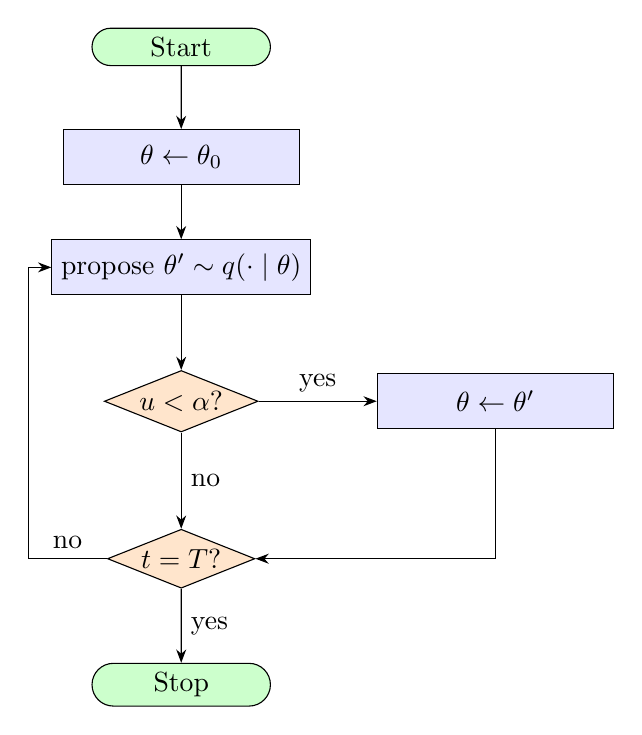
\begin{tikzpicture}[node distance=1.4cm, >=Stealth, start/.style={rounded rectangle, draw, fill=green!20, minimum width=2.5cm}, proc/.style={rectangle, draw, fill=blue!10, minimum width=3cm, minimum height=7mm}, dec/.style={diamond, draw, fill=orange!20, aspect=2.5, inner sep=1pt}]
\node[start] (s) {Start};
\node[proc, below of=s] (init) {$\theta \gets \theta_0$};
\node[proc, below of=init] (prop) {propose $\theta' \sim q(\cdot \mid \theta)$};
\node[dec, below of=prop, yshift=-0.3cm] (acc) {$u < \alpha$?};
\node[proc, right=1.5cm of acc] (keep) {$\theta \gets \theta'$};
\node[dec, below of=acc, yshift=-0.6cm] (done) {$t = T$?};
\node[start, below of=done, yshift=-0.2cm] (e) {Stop};
\draw[->] (s) -- (init); \draw[->] (init) -- (prop); \draw[->] (prop) -- (acc);
\draw[->] (acc) -- node[above] {yes} (keep); \draw[->] (keep) |- (done);
\draw[->] (acc) -- node[right] {no} (done); \draw[->] (done) -- node[right] {yes} (e);
\draw[->] (done.west) -- node[above] {no} ++(-1,0) |- (prop.west);
\end{tikzpicture}
\end{document}
